\subsection{Table reservation}
\begin{enumerate}
    \item Use-case diagram
    \begin{center}
        \begin{figure}[!h]
            \begin{center}
                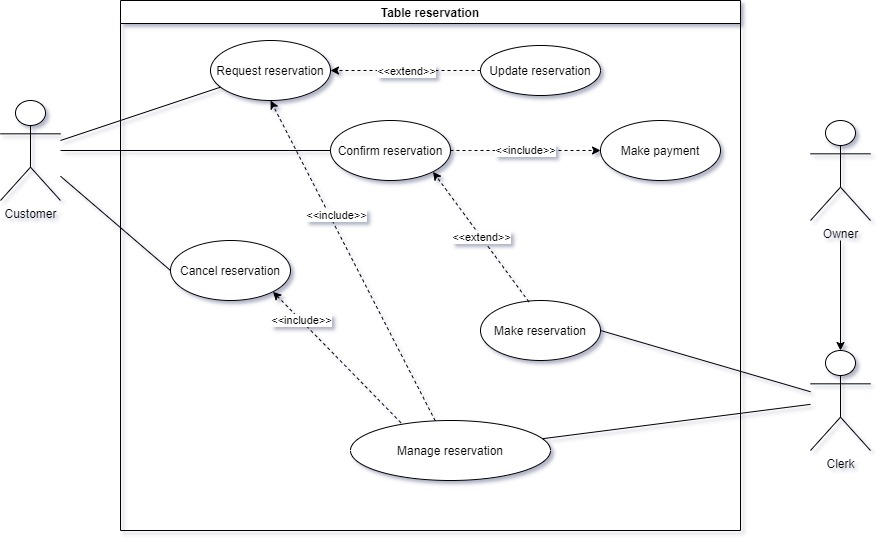
\includegraphics[scale=0.45]{Images/ReservationDiagram.jpg}
            \end{center} 
            \vspace{1cm}
            \caption{Table reservation's use-case diagram}
        \end{figure}    
    \end{center}
    
    \item Use-case make reservation
    \begin{center}{\color{black}}

    \begin{tabular}{|p{5cm}|p{7cm}|} \hline
        Tên usecase &  Request reservation.\\ \hline
        Actor & Khách hàng. \\\hline
        Mô tả & Người dùng sử dụng Request reservation để truy cập ứng dụng web đặt bàn.\\\hline
        Tiền điều kiện & Người dùng phải đăng nhập vào được hệ thống.\\ \hline
        Hậu điều kiện &  Người dùng đã xác nhận đặt bàn và có thông báo được gửi đến.
        \\ \hline
        Luồng điều kiện chính &  
            \begin{enumerate}[1.]
                \item Hệ thống hiển thị giao diện đặt bàn.
                \item Người dùng chọn chức năng  đặt chỗ.
                \item Người dùng xác nhận liệu đó có phải là lần đầu tiên họ ghé thăm nhà hàng.
                
                \item Một biểu mẫu bật lên hỏi người dùng một vài chi tiết cơ bản như tên, chi tiết liên hệ,...
                
			    
            \end{enumerate}\\\hline
        
    \end{tabular}
\end{center}


\begin{center}{\color{black}}

    \begin{tabular}{|p{5cm}|p{7cm}|} \hline
        
        Luồng điều kiện chính &  
            \begin{enumerate}
                \item[5.] Hệ thống hiển thị biểu đồ đặt chỗ ở định dạng bảng (các hàng và cột là thời gian và các ngày trong tuần).
                \item[6.] Người dùng chọn khung thời gian trống và phạm vi giá trong biểu đồ đặt chỗ.
                
				\item[7.] Người dùng đưa ra lựa chọn: Xác nhận/Thay đổi. Nếu xác nhận, hệ thống chuyển sang bước 8. Nếu thay đổi, người dùng thực hiện lại bước 6.
			
				\item[8.] Người dùng tiến hành thanh toán tiền cọc.
				\item[9.] Hệ thống ghi nhận đặt chỗ thành công.
			
            \end{enumerate}\\\hline
        
        Luồng sự kiện phụ &  
                \begin{itemize}
                    \item Thêm chỗ đặt bàn mới.
                    \begin{enumerate}[1.]
                        \item Hệ thống hiển thị giao diện đặt bàn.
                        \item Người dùng chọn khung thời gian phù hợp.
                        \item Người dùng xác nhận thêm chỗ đặt mới.
                    \end{enumerate}
                    \item Xóa chỗ đặt cũ
                    \begin{enumerate}[1.]
                        \item Hệ thống hiển thị các chỗ đặt có thể xóa.
                        \item Người dùng chọn chỗ đặt cần xóa.
                        \item Người dùng xác nhận xóa chỗ đặt
                    \end{enumerate}
                \end{itemize}\\ \hline
    \end{tabular}
\end{center}


    \newpage
    \item Use-case Update reservation
    \begin{center}{\color{black}}
        \begin{tabular}{|p{5cm}|p{7cm}|} \hline
    
        
        Tên usecase &  Update reservation.\\ \hline
        Actor & Khách hàng.\\ \hline
        Mô tả & Người dùng sử dụng Update reservation để truy cập ứng dụng web chỉnh sửa đơn đặt sau khi đã đặt bàn.\\ \hline
        Tiền điều kiện 
        & Người dùng đã đăng nhập vào hệ thống và  đặt bàn  trong vòng 1 giờ.\\ \hline
        
        
        Hậu điều kiện &  Người dùng đã xác nhận  và có thông báo được gửi đến.
                \\ \hline
        Luồng điều kiện chính &  
            \begin{enumerate}[1.]
                \item Người dùng chỉnh sửa các chỗ đã được đặt.
                
                \item Hệ thống hiển thị biểu đồ đặt chỗ. 
                \item Người dùng chọn khung thời gian trống và phạm vi giá trong biểu đồ đặt chỗ hoặc xóa các chỗ đã đặt trước đó.
                
				\item Người dùng đưa ra lựa chọn: Xác nhận/Thay đổi. Nếu xác nhận, hệ thống chuyển sang bước 5. Nếu thay đổi, người dùng thực hiện lại bước 3.
				
				\item Người dùng tiến hành thanh toán tiền cọc.
				\item Hệ thống ghi nhận đặt chỗ thành công.
			
            \end{enumerate}\\
         
        \hline
       
        
    \end{tabular}
    \end{center}




\end{enumerate}

